\section{Aplikacja mobilna - kontroler}

\begin{center}
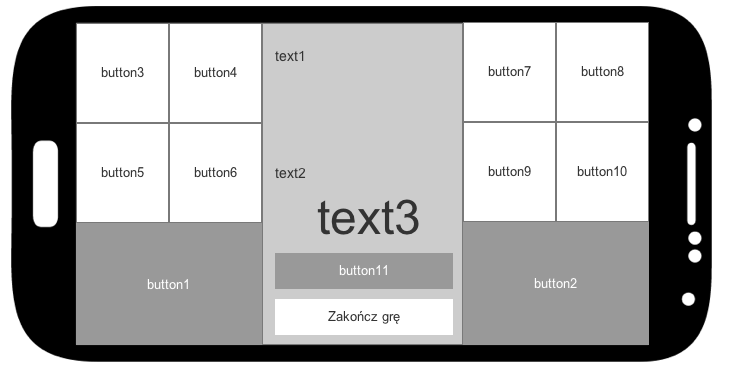
\includegraphics[width=1\textwidth]{images/button_mockup.png}
\captionof{figure}{
Makieta - układ przycisków
}
\end{center}
\paragraph{}
Głównym założeniem było stworzenie uniwersalnego kontrolera przygotowanego pod dowolny rodzaj gry, bądź innej wizualizacji stworzonej w środowisku Unity. Podczas uruchomienia kontrolera serwer wysyła statusy przycisków oraz pól tekstowych.

\subsection{Przyciski}
\paragraph{}
Każdy przycisk może zostać skonfigurowany poprez ustawienie tekstu. Dodatkowo można zablokować przycisk podczas gdy nie jest on potrzebny w danym czasie.
\paragraph{}
Aby ułatwić pracę nad aplikacją stworzono pole wyliczalne (ENUM) zawierającą wszystkie przyciski.

\begin{lstlisting}[language=Java]
public enum ButtonEnum {
    BTN1, BTN2, BTN3, BTN4, BTN5, BTN6, BTN7, BTN8, BTN9, BTN10, BTN11
}
\end{lstlisting}
\captionof{lstlisting}{
	Enum z przyciskami
}
\paragraph{}
Jednakże aby powiązać elementy ,,Button'' z warstwy widoku (defincja XML) na kod przycisku  należy stworzyć listę elementów. Będzie ona służyła do wyszukiwania przycisków oraz zmiany ich właściwości. Dodatkowo do każdego przycisku należy dodać obsługę zdarzeń. Po kliknięciu wysyłany będzie odpowiedni komunikat.

\begin{lstlisting}[language=Java]
    protected HashMap<ButtonEnum, Button> buttonsMap = new HashMap<ButtonEnum, Button>();

    protected void mapButton(int btnId, final ButtonEnum btnName) {
        final Button button = (Button) findViewById(btnId);
        buttonsMap.put(btnName, button);

        button.setOnClickListener(new View.OnClickListener() {
            public void onClick(View v) {
                sendToServer("button_" + btnName);
            }
        });
    }
\end{lstlisting}
\captionof{lstlisting}{
	Metoda obsługująca przycisk
}


\begin{lstlisting}[language=Java]
 @Override
    protected void onCreate(Bundle savedInstanceState) {
        super.onCreate(savedInstanceState);

        this.mapButton(R.id.button1, ButtonEnum.BTN1);
        this.mapButton(R.id.button2, ButtonEnum.BTN2);

    }
\end{lstlisting}
\captionof{lstlisting}{
	Przykład mapowania przycisku
}

\subsection{Informacje tekstowe}
\paragraph{}
Pola tekstowe mogą mieć ustawioną dowolną treść w dowolnym czasie.

\subsection{Komunikacja sieciowa}
